\section{Experimental Setup and Environmental Protocols}
\label{sec:experimental_setup}

\subsection{Physics Engine Verification: Canonical Orbium Benchmark}
\label{subsec:exp_physics_verification}

To ensure that experimental results reflect authentic physical and evolutionary dynamics rather than numerical drift or algorithmic bugs, the JAX simulation engine is verified against the canonical \textit{Orbium unicaudatus} glider \parencite{chan2019lenia, plantec2025flowlenia}. The Orbium glider is a known, analytically stable soliton solution within continuous cellular automata that maintains steady linear locomotion only when spatial convolutions, continuous growth evaluations, and advection updates are executed with exact numerical fidelity.

The verification benchmark is initialized on a $256 \times 256$ toroidal lattice using decoded Run-Length Encoded (RLE) mass arrays. Canonical physiological parameters are assigned according to the stable glider regime:
\begin{equation}
\mu = 0.150, \quad \sigma = 0.015, \quad \vscale = 5.20, \quad \adiff = 0.060
\label{eq:orbium_parameters}
\end{equation}
The simulation is executed over an isolated horizon of $T = 3000\text{ steps}$. Exact mass conservation is monitored at each time step by tracking the relative mass drift:
\begin{equation}
\Delta M_{\text{rel}}(t) = \frac{\left| \sum_{\mathbf{x}} A(\mathbf{x}, t) - \sum_{\mathbf{x}} A(\mathbf{x}, 0) \right|}{\sum_{\mathbf{x}} A(\mathbf{x}, 0)}
\label{eq:mass_drift_metric}
\end{equation}
This standalone verification serves as a positive control, providing evidence that the spectral Fourier solver and semi-Lagrangian bilinear advection scheme \parencite{moroz2020reintegration} operate with machine-level precision before introducing evolutionary exploration or environmental obstacles.

\subsection{Genome-Mixing Rule Ablation Protocols}
\label{subsec:exp_mixing_ablations}

To evaluate how genetic collision operators affect multi-species evolutionary dynamics and prevent parameter homogenization, two distinct ablation setups are tested across $T = 3600\text{ steps}$ on a $256 \times 256$ domain seeded with $S = 6$ interacting Gaussian patches:

\begin{enumerate}
    \item \textbf{Ablation A (Stochastic Gene-Wise Sampling):} Lineages interact via Gumbel-Max categorical sampling over incoming directional mass fluxes (\Cref{eq:gumbel_max_mixing}). Periodic local mutations ($\sigma_{\text{mut}} = 0.01, R_{\text{mut}} = 10\text{ px}$) are applied every $T_{\text{mut}} = 50\text{ steps}$.
    \item \textbf{Ablation B (Softmax Growth Negotiation):} Overlapping parameter fields are updated dynamically via temperature-scaled competitive growth negotiation (\Cref{eq:softmax_negotiation}) across aggressiveness values $\beta \in \{1.0, 2.0, 3.0, 4.0\}$.
\end{enumerate}

These ablations quantify the degree to which discrete parameter sampling versus continuous growth competition preserves phenotypic diversity and prevents collapse into undifferentiated parameter averages.

\subsection{Curiosity-Driven Discovery vs. Uniform Random Search}
\label{subsec:exp_imgep_vs_random}

To evaluate the exploration efficiency of Intrinsically Motivated Goal Exploration Processes (IMGEP), we establish a comparative benchmark against an unguided Uniform Random Search baseline:

\begin{itemize}
    \item \textbf{IMGEP Exploration:} Executes $N_{\text{trials}} = 50$ iterations per run, beginning with $N_{\text{bootstrap}} = 10$ uniform bootstrap rollouts. Subsequent trials sample random behavioral goals uniformly across the 3D metric bounds:
    \begin{equation}
    \Motility \in [0.0, 150.0]\text{ px}, \quad \EvoActivity \in [0.0, 0.050], \quad \Complexity \in [0, 50000]\text{ bytes}
    \label{eq:metric_bounds}
    \end{equation}
    Parents are selected via nearest-neighbor Euclidean distance in normalized metric space, followed by Gaussian genome perturbation ($\sigma_{\text{mut}} = 0.010$).
    \item \textbf{Uniform Random Search Baseline:} Samples all $N_{\text{trials}} = 50$ candidate genomes independently and uniformly from the full hyperparameter bounding box ($\mu_k \in [0.10, 0.28]$, $\sigma_k \in [0.008, 0.030]$, $R_k \in [6.0, 15.0]\text{ px}$).
\end{itemize}

Both search regimes are evaluated under the five-stage watertight quality filter across three independent pseudo-random seeds ($\text{seeds} \in \{42, 101, 2024\}$) to ensure statistical validity.

\subsection{Chemotactic Foraging and Cohesion-Fission Assay}
\label{subsec:exp_chemotaxis_protocol}

To study soft-bodied locomotion and surface tension under active directional forces, an open toroidal domain ($256 \times 256$) is configured with a static horizontal nutrient gradient $R(\mathbf{x})$:
\begin{equation}
R(y, x) = \frac{x}{W - 1} \in [0.0, 1.0]
\label{eq:chemotaxis_ramp}
\end{equation}
Organisms are initialized at the nutrient-poor left boundary ($x_0 = 50\text{ px}$) facing an attractive gradient toward the nutrient-rich right boundary ($x_{\text{target}} = 200\text{ px}$). The total advection velocity field couples continuous growth gradients to the external chemotactic pull:
\begin{equation}
\mathbf{v}_{\text{total}}(\mathbf{x}) = \vscale \cdot \Big( (1 - \adiff) \nabla G(U)(\mathbf{x}) - \adiff \nabla A(\mathbf{x}) \Big) + \chi \cdot \nabla R(\mathbf{x})
\label{eq:chemotaxis_velocity_coupling}
\end{equation}
\begin{equation}
\mathbf{v}_{\text{bounded}}(\mathbf{x}) = \tanh\left( \mathbf{v}_{\text{total}}(\mathbf{x}) \right)
\label{eq:chemotaxis_velocity_bounded}
\end{equation}

A systematic parameter sweep is conducted across chemotactic sensitivity $\chi \in [0.0, 25.0]$, diffusion regularizer $\adiff \in [0.030, 0.080]$, and growth tolerance $\sigma \in [0.010, 0.020]$ to map the boundary between cohesive droplet migration, structural tearing, and amoeboid fission.

\subsection{Soft-Bodied Barrier Constriction Assay}
\label{subsec:exp_barrier_constriction}

To quantify the mechanical elasticity of Flow Lenia solitons encountering rigid geometric obstacles, we formulate a two-chamber barrier constriction assay (\Cref{fig:diagram_barrier_constriction_setup}).

A solid, impermeable vertical wall of thickness $d = 8\text{ pixels}$ is placed at $x = W/2 = 128\text{ pixels}$, partitioning the lattice into:
\begin{itemize}
    \item \textbf{Chamber 1 (Spawn Zone, $x < 124$):} Initial spawn region where a cohesive soliton is initialized at $(y_0, x_0) = (128, 50)$ with an equilibrium radius of $r_0 = 14.0\text{ pixels}$.
    \item \textbf{Chamber 2 (Target Reservoir, $x > 132$):} Destination chamber containing a rich nutrient pool.
\end{itemize}

A central passage corridor of width $W_{\text{passage}}$ connects the two chambers:
\begin{equation}
\EnvMask(y, x) = 
\begin{cases}
1.0 & \text{if } |x - 128| > 4 \quad (\text{Chamber interiors}) \\
1.0 & \text{if } |x - 128| \le 4 \text{ and } |y - 128| \le \frac{W_{\text{passage}}}{2} \quad (\text{Aperture corridor}) \\
0.0 & \text{otherwise} \quad (\text{Rigid barrier wall})
\end{cases}
\label{eq:barrier_mask_definition}
\end{equation}

\begin{figure}[htbp]
\centering
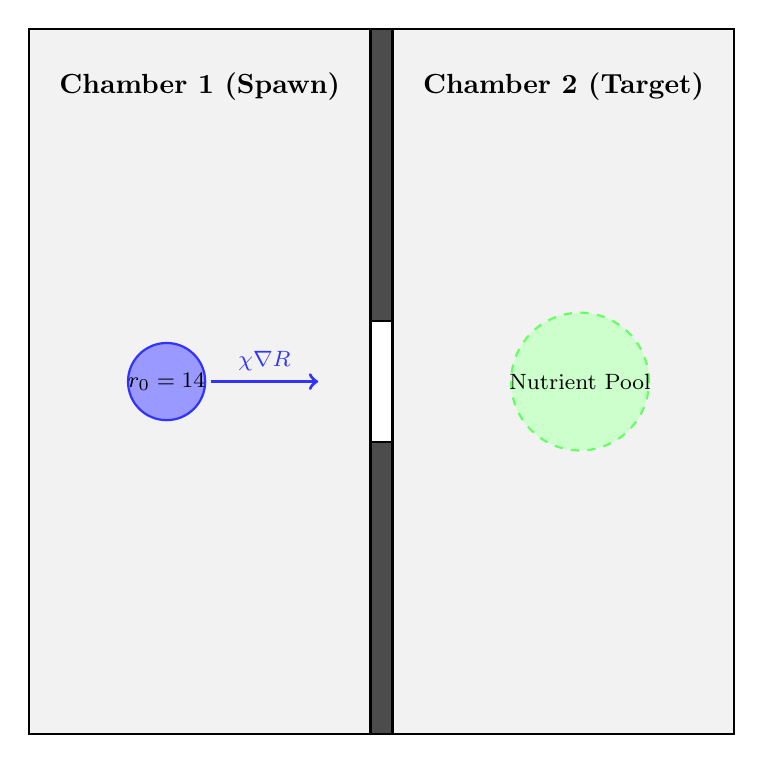
\begin{tikzpicture}[scale=0.035]
    % Chamber 1
    \draw[thick, fill=gray!10] (0, 0) rectangle (124, 256);
    \node at (62, 235) {\textbf{Chamber 1 (Spawn)}};
    % Soliton initial
    \draw[fill=blue!40, draw=blue!80, thick] (50, 128) circle (14);
    \node at (50, 128) {\footnotesize $r_0=14$};
    \draw[->, very thick, blue!80] (66, 128) -- (105, 128) node[midway, above] {\footnotesize $\chi \nabla R$};
    
    % Barrier Wall Top
    \draw[thick, fill=black!70] (124, 150) rectangle (132, 256);
    % Barrier Wall Bottom
    \draw[thick, fill=black!70] (124, 0) rectangle (132, 106);
    
    % Corridor
    \draw[<->, thick, red] (136, 106) -- (136, 150) node[midway, right] {\footnotesize $W_{\text{passage}}$};
    
    % Chamber 2
    \draw[thick, fill=gray!10] (132, 0) rectangle (256, 256);
    \node at (194, 235) {\textbf{Chamber 2 (Target)}};
    \draw[fill=green!20, draw=green!60, dashed, thick] (200, 128) circle (25);
    \node at (200, 128) {\footnotesize Nutrient Pool};
\end{tikzpicture}
\caption{Schematic diagram of the soft-bodied barrier constriction assay. A solid barrier of thickness $d = 8\text{ px}$ separates Chamber 1 from Chamber 2, connected exclusively by an aperture of width $W_{\text{passage}}$.}
\label{fig:diagram_barrier_constriction_setup}
\end{figure}

The transmission coefficient $T(W_{\text{passage}})$ measures the fraction of total initial mass successfully transported into Chamber 2 by the end of the simulation horizon ($T = 3600\text{ steps}$):
\begin{equation}
T(W_{\text{passage}}) = \frac{\sum_{y=0}^{H-1} \sum_{x = W/2 + 4}^{W-1} A(\mathbf{x}, t_{\text{end}})}{\sum_{\mathbf{x}} A(\mathbf{x}, 0)} \times 100\%
\label{eq:transmission_coefficient_def}
\end{equation}
Aperture widths are evaluated systematically across $W_{\text{passage}} \in \{8, 16, 24, 32, 48, 64\}\text{ pixels}$ under seeds $\{42, 101, 2024\}$.

\subsection{Dynamic Resource Depletion and Niche Construction}
\label{subsec:exp_resource_depletion}

To simulate reciprocal niche construction, organisms interact with a dynamic, stateful scalar resource field $R(\mathbf{x}, t) \in [0.0, 1.0]$. The resource field evolves according to local organism density:

\begin{equation}
R(\mathbf{x}, t + \Delta t) = 
\begin{cases}
\max\Big(0.0, \, R(\mathbf{x}, t) - \delta_{\text{dep}}\Big) & \text{if } A(\mathbf{x}, t) \ge 0.10 \quad (\text{Consumption}) \\
\min\Big(1.0, \, R(\mathbf{x}, t) + \delta_{\text{reg}}\Big) & \text{if } A(\mathbf{x}, t) < 0.10 \quad (\text{Regeneration})
\end{cases}
\label{eq:resource_depletion_dynamics}
\end{equation}
where $\delta_{\text{dep}} = 0.04$ defines the per-step depletion rate and $\delta_{\text{reg}} = 0.01$ denotes the slower replenishment rate.

The local growth potential is directly modulated by available resources:
\begin{equation}
\EffectiveGrowth(\mathbf{x}, t) = G(U)(\mathbf{x}, t) \cdot R(\mathbf{x}, t)
\label{eq:coupled_growth_depletion}
\end{equation}
This establishes a negative feedback mechanism: stationary organisms deplete their immediate environment, causing their effective growth potential to drop and forcing active migration to avoid structural collapse.

\subsection{Macro-Scale Ecology: Multi-Chamber Ecological Arena Benchmark}
\label{subsec:exp_colosseum_ecosystem}

To evaluate whether Flow Lenia dynamics scale across larger spatial domains and extended temporal horizons, we design a multi-chamber arena benchmark (\Cref{fig:diagram_colosseum_arena}).

The arena features:
\begin{itemize}
    \item \textbf{Simulation Grid:} High-resolution domain ($384 \times 384$ and $512 \times 512$ lattice sites) simulated over an extended horizon of $T = 22500\text{ continuous steps}$.
    \item \textbf{Initial Population:} $S = 8$ distinct species lineages initialized at peripheral coordinates with randomized physiological genomes $(\boldsymbol{\mu}_s, \boldsymbol{\sigma}_s, \mathbf{w}_s)$.
    \item \textbf{Spatial Architecture:} Four quadrant resource sanctuaries positioned symmetrically around a central circular arena with cardinal passage archways.
    \item \textbf{Cyclic Grazing Dynamics:} Resource fields operate with balanced depletion ($\delta_{\text{dep}} = 0.004$) and slow regeneration ($\delta_{\text{reg}} = 0.001$), coupled with periodic gate transitions every $2500\text{ steps}$.
\end{itemize}

\begin{figure}[htbp]
\centering
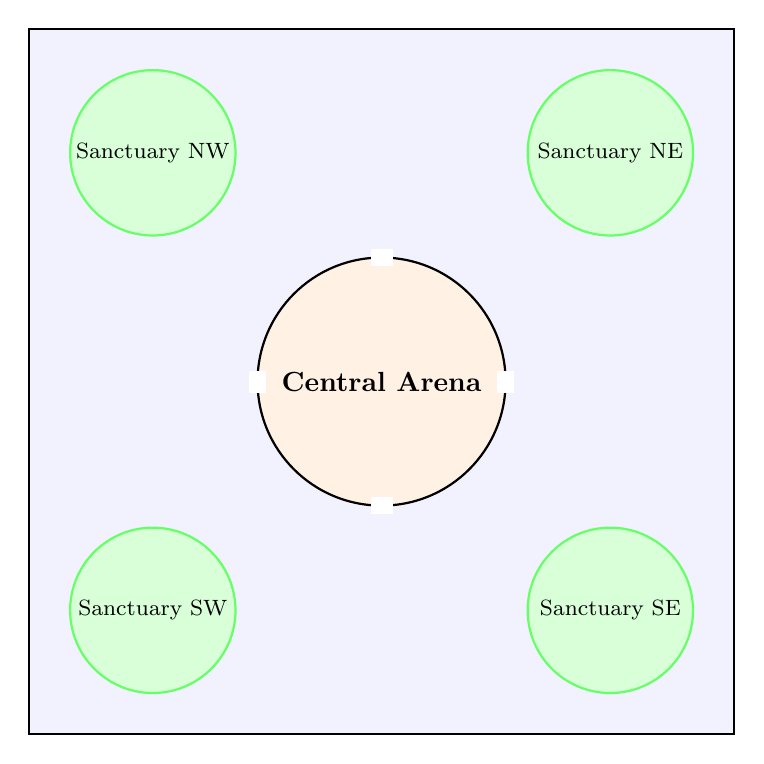
\begin{tikzpicture}[scale=0.035]
    % Outer boundary
    \draw[thick, fill=blue!5] (0,0) rectangle (256,256);
    % Four Sanctuaries
    \draw[thick, fill=green!15, draw=green!60] (45,45) circle (30);
    \node at (45,45) {\footnotesize Sanctuary SW};
    \draw[thick, fill=green!15, draw=green!60] (211,45) circle (30);
    \node at (211,45) {\footnotesize Sanctuary SE};
    \draw[thick, fill=green!15, draw=green!60] (45,211) circle (30);
    \node at (45,211) {\footnotesize Sanctuary NW};
    \draw[thick, fill=green!15, draw=green!60] (211,211) circle (30);
    \node at (211,211) {\footnotesize Sanctuary NE};
    % Central Arena
    \draw[thick, fill=orange!10, draw=black] (128,128) circle (45);
    \node at (128,128) {\textbf{Central Arena}};
    % Cardinal Gates
    \draw[fill=white, draw=none] (124, 170) rectangle (132, 176);
    \draw[fill=white, draw=none] (124, 80) rectangle (132, 86);
    \draw[fill=white, draw=none] (80, 124) rectangle (86, 132);
    \draw[fill=white, draw=none] (170, 124) rectangle (176, 132);
\end{tikzpicture}
\caption{Spatial layout of the multi-chamber ecological arena benchmark ($384 \times 384$). Four peripheral nutrient sanctuaries surround a central arena accessible through cardinal archways.}
\label{fig:diagram_colosseum_arena}
\end{figure}

\subsection{Hardware Architecture and Multi-Seed Protocol}
\label{subsec:exp_hardware_protocol}

All simulations are executed in native functional JAX compiled via Google XLA (Accelerated Linear Algebra). Time-steppers are mapped to compiled loop graphs via \texttt{jax.lax.scan}, entirely eliminating Python runtime overhead.

To ensure computational reproducibility and account for stochastic initialization variance, all core experiments are evaluated across three fixed pseudo-random seeds ($\text{PRNG seeds} = \{42, 101, 2024\}$). Hardware configurations, execution times, and memory allocations are summarized in \Cref{tab:hardware_resource_matrix}.

\begin{table}[htbp]
\centering
\footnotesize
\caption{Computational Resource Allocation and Simulation Throughput across Experimental Groups.}
\label{tab:hardware_resource_matrix}
\begin{tabularx}{\textwidth}{X ccccc}
\toprule
\textbf{Experimental Group} & \textbf{Grid Size} & \textbf{Horizon ($T$)} & \textbf{Concurrency} & \textbf{Throughput} & \textbf{VRAM (MB)} \\
\midrule
Orbium Verification & $256 \times 256$ & $3000\text{ steps}$ & $N = 1$ & $33300\text{ steps/s}$ & $\sim 240$ \\
Gene-Wise Mixing Ablation & $256 \times 256$ & $3600\text{ steps}$ & $N = 1$ & $28500\text{ steps/s}$ & $\sim 310$ \\
IMGEP Goal Discovery & $256 \times 256$ & $2000\text{ steps}$ & $N = 16$ (\texttt{vmap}) & $24200\text{ steps/s}$ & $\sim 1450$ \\
Barrier Constriction ($T(W)$) & $256 \times 256$ & $3600\text{ steps}$ & $N = 6$ (\texttt{vmap}) & $29100\text{ steps/s}$ & $\sim 820$ \\
Resource Depletion & $256 \times 256$ & $3600\text{ steps}$ & $N = 1$ & $26800\text{ steps/s}$ & $\sim 340$ \\
Colosseum Grand Synthesis & $384 \times 384$ & $22500\text{ steps}$ & $N = 1$ & $18400\text{ steps/s}$ & $\sim 680$ \\
Scale-Up Invariance & $512 \times 512$ & $3600\text{ steps}$ & $N = 1$ & $11200\text{ steps/s}$ & $\sim 940$ \\
\bottomrule
\end{tabularx}
\end{table}